\documentclass{rvcepaper}
% s7-common.tex -- macros shared by the Sem 7 CIE papers (\input right after \documentclass{rvcepaper})
% placeholder for text that cannot be read in the scan
\newcommand{\illeg}{\textit{[illegible]}}
\newcommand{\illegc}{{\tiny\textit{[illegible]}}}
% question table with a custom header row: \begin{gtable}[PART -- A]{Sl.\newline No.}{Questions}{M}{BT}{CO}
% the optional title is set as the table's first row so it never strands at a page foot
\newcommand{\gtitlerow}{}
\newenvironment{gtable}[6][]{%
  \def\gtitle{#1}\ifx\gtitle\empty\def\gtitlerow{}\else\def\gtitlerow{\multicolumn{5}{c}{\bfseries\gtitle}\\*[2pt]}\fi
  \begin{longtable}{|C{1.05cm}|p{12.2cm}|C{0.95cm}|C{0.95cm}|C{0.95cm}|}
  \gtitlerow
  \hline \textbf{#2} & \multicolumn{1}{c|}{\textbf{#3}} & \textbf{#4} & \textbf{#5} & \textbf{#6}\\* \hline
  \endfirsthead
  \endhead
}{\end{longtable}}
\newcommand{\twonotes}[2]{{\small Note:}\par\vspace{-1pt}
\hspace*{0.5cm}{\footnotesize 1. \hspace{0.1cm}#1}\par
\hspace*{0.5cm}{\footnotesize 2. \hspace{0.1cm}#2}\par\vspace{3pt}}
\newcommand{\onenote}[1]{{\small Note:}\par\vspace{-1pt}
\hspace*{0.5cm}{\footnotesize 1. \hspace{0.1cm}#1}\par\vspace{3pt}}
% keep the BT/CO caption and the marks-distribution table on the same page
\renewcommand{\btfoot}[2]{\par\vspace{8pt}\noindent\begin{minipage}{\textwidth}\centering
  {\small BT-Blooms Taxonomy, CO-Course Outcomes, M-Marks}\par\vspace{2pt}
  \begin{tabular}{#1}#2\end{tabular}\end{minipage}\par\nopagebreak\vspace{2pt}}
\newcommand{\xfoot}[3]{\par\vspace{8pt}\noindent\begin{minipage}{\textwidth}\centering
  {\small #1}\par\vspace{2pt}\begin{tabular}{#2}#3\end{tabular}\end{minipage}\par\nopagebreak\vspace{2pt}}
\newcommand{\qq}[5]{#1 & #2 & #3 & #4 & #5\\}
\newcommand{\qm}[3]{#1 & #2 & #3\\ \hline}
% other-department header table (Date / Course Code / Sem rows + title row)
\newcommand{\ofour}[7]{\noindent\begingroup\renewcommand{\arraystretch}{1.3}\fontsize{11.5}{13}\selectfont
\begin{tabular}{|C{3.6cm}|C{4.6cm}|C{4.0cm}|C{3.8cm}|}\hline
Date & #1 & Maximum Marks & #2\\\hline
Course Code & #3 & Duration & #4\\\hline
Sem & #5 & \multicolumn{2}{c|}{#6}\\\hline
\multicolumn{4}{|c|}{\bfseries\fontsize{13}{15}\selectfont #7}\\\hline
\end{tabular}\endgroup\par\vspace{6pt}}
\renewcommand{\arraystretch}{1.05}
% the closing stars line stays with the block above it
\renewcommand{\stars}[1]{\par\nopagebreak\vspace{2pt}\nopagebreak\centerline{#1}}
% printed value struck through by hand, with the handwritten correction under it: \corr{60}{34}
\usepackage[normalem]{ulem}
\newcommand{\corr}[2]{\shortstack{\sout{#1}\\#2}}
\usetikzlibrary{decorations.pathmorphing}
% "Academic year" header table without the DEPARTMENT OF block (use inside iempaperB after \paperinfo)
\newcommand{\iemtableB}{%
  \par\vspace{4pt}\noindent\begingroup\renewcommand{\arraystretch}{1.5}\bfseries\fontsize{11.5}{13}\selectfont
  \begin{tabular}{|p{4.2cm}|p{5.0cm}|p{3.7cm}|p{3.6cm}|}\hline
   Date & \getkey{date} & Maximum Marks & \getkey{maxmarks}\\\hline
   Course Code & \getkey{code} & Duration & \getkey{duration}\\\hline
   Sem & \getkey{sem} & \multicolumn{2}{l|}{\getkey{exam}}\\\hline
   \multicolumn{4}{|c|}{\getkey{title}}\\\hline
  \end{tabular}\endgroup\par\vspace{4pt}}
% other-department CIE header: \xdept{Department line}{left1}{mid1}{right1}{left2}{mid2}{right2}{course title cell}{right3}
\newcommand{\xdept}[9]{\par\vspace{2pt}\centerline{\bfseries\fontsize{13.5}{16}\selectfont #1}\par\vspace{4pt}
  \noindent\begingroup\renewcommand{\arraystretch}{1.5}\bfseries\fontsize{11.5}{13}\selectfont
  \begin{tabular}{|p{4.8cm}|C{5.6cm}|p{5.7cm}|}\hline
  #2 & #3 & #4\\\hline #5 & #6 & #7\\\hline \multicolumn{2}{|p{10.8cm}|}{#8} & #9\\\hline
  \end{tabular}\endgroup\par\vspace{8pt}}

\begin{document}

% ---------- 21HS71 Constitution of India and Professional Ethics
\begin{iempaperB}
\paperinfo{ayear={2024-2025 (ODD Sem)},date={27th January 2025},code={21HS71},sem={VII Semester},exam={CIE -- II},maxmarks={10 + 50},duration={120 Mins},
 title={CONSTITUTION OF INDIA AND PROFESSIONAL ETHICS},shownote=0}
\iemheadB
\onenote{Answer all the Questions.}
\begin{gtable}[PART -- A]{Sl.\newline No.}{Questions}{M}{BT}{CO}
\q{1}{Define Uniform Civil Code.}{02}{2}{2}
\q{2}{List any two powers of National Human Rights Commission (NHRC) .}{02}{2}{2}
\q{3}{What is ``product liability''?}{02}{2}{2}
\q{4}{Differentiate between unfair Trade practice \& Deficiency in Services.}{02}{2}{2}
\q{5}{List any two consumer Rights available under the Act}{02}{2}{2}
\end{gtable}
\begin{gtable}[PART -- B]{Sl.\newline No.}{Questions}{M}{BT}{CO}
\q{1.a}{Examine the Constitutional position of Governor of a State.}{05}{2}{1}
\q{1.b}{Discuss Online shopping and product liability covering-Liability of a product retailer or delivery service and Liability related to online food products.}{05}{2}{1}
\q{2.a}{Explain the Impeachment proceedings of President of India.}{05}{2}{2}
\q{2.b}{Discuss the ground and procedure of removing the Judges of Supreme Court}{05}{3}{2}
\q{3}{List 11 Fundamental Duties enshrined in the Constitution of India.}{10}{2}{1}
\q{4}{The slogan line of ``Jago Grahak Jago'' is applicable today. Discuss the Historical perspective, Significance and Key features of Consumer Protection Act (both old and new).}{10}{3}{2}
\q{5}{Directive principle is fundamental in making Welfare state''. Discuss}{10}{4}{3}
\end{gtable}
\btfoot{|l|l|l|*{5}{C{0.8cm}|}*{6}{C{0.8cm}|}}{\hline
\multirow{3}{*}{Marks Distribution} & \multicolumn{2}{c|}{Particulars} & CO1 & CO2 & CO3 & CO4 & CO5 & L1 & L2 & L3 & L4 & L5 & L6\\\cline{2-14}
 & \multirow{2}{*}{\shortstack{Max\\Marks}} & Quiz & -- & 10 & -- & -- & -- & -- & 10 & -- & -- & -- & --\\\cline{3-14}
 & & Test & 20 & 20 & 10 & - & 25 & 15 & 10 & & - & - & 20\\\hline}
\end{iempaperB}

% ---------- 21IM72 Product Design & Development
\begin{iempaperB}
\paperinfo{ayear={2024-2025 (ODD Sem)},date={27\textsuperscript{th} January 2025},code={21IM72},sem={VII Semester},exam={CIE -- II},maxmarks={10 + 50},duration={120 Mins},
 title={PRODUCT DESIGN \& DEVELOPMENT},shownote=0}
\iemheadB
\twonotes{Answer all the Questions.}{Avoid verbose answers and answer specifically and to the point.}
\begin{gtable}[PART -- A]{Sl.\newline No.}{Questions}{M}{BT}{CO}
\q{1}{What does Design for Cost (DfC) aim to achieve?}{01}{L$_2$}{CO3}
\q{2}{List any two main objectives of Design for Maintainability (DfM)?}{01}{L$_2$}{CO3}
\q{3}{Name one method used in Design for Usability (DfU).}{01}{L$_1$}{CO3}
\q{4}{Mention the purpose of Design for Sustainability (DfS)?}{01}{L$_2$}{CO3}
\q{5}{How does Design for Logistics (DfL) impact the supply chain management?}{01}{L$_2$}{CO3}
\q{6}{What is the focus of Design for Compliance (DfC)?}{01}{L$_1$}{CO4}
\q{7}{Mention Design for Testability (DfT) improve product quality?}{01}{L$_2$}{CO4}
\q{8}{Define ``product backlog'' in agile.}{01}{L$_1$}{CO4}
\q{9}{Which agile role is responsible for maximizing the value of the product?}{01}{L$_1$}{CO4}
\q{10}{Mention any one feature of the stage gate product development process.}{01}{L$_2$}{CO4}
\end{gtable}
\begin{gtable}[PART -- B]{Sl.\newline No.}{Questions}{M}{BT}{CO}
\q{1.}{Explain the principles of Design for Assembly (DfA). How does DfA impact the efficiency and cost of product assembly? Use case studies or examples to support your answer.}{10}{L$_3$}{CO3}
\q{2.}{A company is developing a new eco-friendly packaging solution. Evaluate how Design for Sustainability (DfS) principles can be integrated into their product development process and the potential impact on their brand and market position.}{10}{L$_4$}{CO4}
\q{3.}{A consumer electronics company is launching a new smartphone and wants to ensure it is easy to assemble and test. Discuss how Design for Assembly (DfA) and Design for Testability (DfT) principles can be applied to achieve these goals.}{10}{L$_4$}{CO4}
\q{4.}{A global automotive company is developing an electric vehicle. Discuss how they can incorporate Design for Cost (DfC) and Design for Sustainability (DfS) principles to ensure the vehicle is affordable and environmentally friendly.}{10}{L$_4$}{CO4}
\q{5.}{Discuss the advantages and disadvantages of using the agile product development approach in a fast-paced technology environment. Provide examples to support your arguments.}{10}{L$_3$}{CO3}
\end{gtable}
\btfoot{|l|l|l|*{5}{C{0.8cm}|}*{6}{C{0.8cm}|}}{\hline
\multirow{3}{*}{Marks Distribution} & \multicolumn{2}{c|}{Particulars} & CO1 & CO2 & CO3 & CO4 & CO5 & L1 & L2 & L3 & L4 & L5 & L6\\\cline{2-14}
 & \multirow{2}{*}{\shortstack{Max\\Marks}} & Quiz & - & - & 05 & 05 & -- & 4 & 6 & - & -- & -- & --\\\cline{3-14}
 & & Test & & & 20 & 30 & -- & -- & -- & 20 & 30 & & --\\\hline}
\stars{***********}
\end{iempaperB}

% ---------- 21IM74HD Database Management System
\begin{iempaperB}
\paperinfo{ayear={2024-2025 (Odd Sem)},usn=0,date={29\textsuperscript{th} January 2025},code={21IM74HD},sem={VII},exam={CIE -- II},maxmarks={50 + 10},duration={90 + 20 Min},
 title={DATABASE MANAGEMENT SYSTEM},shownote=0}
\iemheadB
{\small Note: Answer all the Questions.}\par\vspace{3pt}
\begin{gtable}{Sl No}{Questions}{M}{BT}{CO}
\qpart{Part A}
\q{1.}{Enumerate the three types of relationship that exists between entities in an ER diagram.}{02}{L1}{CO2}
\q{2.}{Mention the need for defining Database constraints in DBMS.}{02}{L4}{CO1}
\q{3.}{List the features of Foreign Key.}{02}{L2}{CO3}
\q{4.}{PROJECT is Unary operation. Justify}{02}{L4}{CO3}
\q{5.}{Consider the following schema of relations:\newline
\textit{Student (ssn, name, address, major)}\newline
\textit{Course (code, title)}\newline
\textit{Registered (ssn,code)}\newline
Write an appropriate query for listing the codes of courses in which at least one student is registered (registered courses).}{02}{L3}{CO4}
\qpart{Part B}
\q{1 a}{Consider the following schema:\newline
Suppliers (sid : integer, sname : string, address :string)\newline
Parts (pid : integer, pname : string, color : string)\newline
Catalog (sid : integer,pid : integer, cost : real)
\begin{romi}\item Find the name of suppliers who supply some red parts\item Find the sids of suppliers who supply every part\end{romi}}{05}{L3}{CO4}
\q{b}{Explain the integrity constraints: Not Null, Primary Key with an example each. Is the combination `Not Null, Primary Key' a valid combination? Justify.}{05}{L4}{CO3}
\q{2}{Illustrate different types of Constraints in DBMS with examples.}{10}{L3}{CO1}
\q{3}{``Whenever update operations are applied on the relations, it is necessary that the integrity constraints are not violated''. Evaluate the statement with relevant examples.}{10}{L4}{CO3}
\q{4}{Consider the following relation, BOOK.
\qtabc{l|c|c|l}{\textbf{BOOK} & \textbf{Acc-No} & \textbf{Yr-Pub} & \multicolumn{1}{c}{\textbf{Title}}\\\cline{2-4}
 & 734216 & 1982 & Supply Chain Management\\\cline{2-4}
 & 237235 & 1995 & Database design\\\cline{2-4}
 & 631523 & 1992 & Machine design\\\cline{2-4}
 & 543211 & 1991 & Quality Management\\\cline{2-4}
 & 376112 & 1992 & Personnel Management\\}
Write the syntax for applying the following queries on the relation, BOOK.
\begin{abc}\item Select from the relation, BOOK all the books whose year of publication is 1992.\item Select from the relation, BOOK all the books whose Acc-No is greater than or equal to 56782.\item List all the Title and Acc-no of the BOOK relation.\end{abc}
List all the Title and Yr-Pub of the BOOK relation}{10}{L3}{CO4}
\q{5}{From the relations R and S , find the following:\newline
(a) R $\cup$ S \qquad (b) R $\cap$ S \quad (c) \ R -- S \qquad (d) S -- R\par\vspace{4pt}
\centerline{\begin{tabular}{c|c|c}\textbf{R} & \textbf{Sl.No} & \textbf{DEPT}\\\cline{2-3} & S1 & PHYS1\\\cline{2-3} & S2 & PSY\\\cline{2-3} & S3 & CHEM\\\cline{2-3} & S4 & JOUR\\\end{tabular}\hspace{1.5cm}%
\begin{tabular}{c|c|c}\textbf{S} & \textbf{Sl.No} & \textbf{DEPT}\\\cline{2-3} & S10 & MATH1\\\cline{2-3} & S3 & CHEM\\\cline{2-3} & S15 & ENG\\\cline{2-3} & S16 & MATH2\\\end{tabular}}\par\vspace{2pt}\nointerlineskip\hbox{}}{10}{L4}{\illegc}
\end{gtable}
\btfoot{|l|l|l|*{5}{C{0.8cm}|}*{6}{C{0.8cm}|}}{\hline
\multirow{3}{*}{\shortstack{Marks\\Distribution}} & \multicolumn{2}{c|}{Particulars} & CO1 & CO2 & CO3 & CO4 & CO5 & L1 & L2 & L3 & L4 & L5 & L6\\\cline{2-14}
 & Quiz & \multirow{2}{*}{Max Marks} & 2 & 2 & 4 & 2 & - & 02 & 02 & 02 & 04 & - & -\\\cline{2-2}\cline{4-14}
 & Test & & 10 & - & 15 & 25 & - & - & - & 25 & 25 & - & -\\\hline}
\stars{***}
\end{iempaperB}

% ---------- 21IM74HA Facilities Planning and Design
\begin{iempaperB}
\paperinfo{ayear={2024-2025 (ODD Sem)},usn=0,date={28.01.2025},code={21IM74HA},sem={VII},exam={CIE -- II},maxmarks={10+50},duration={30+90 Min},
 title={FACILITIES PLANNING and DESIGN},shownote=0}
\iemheadB
\onenote{Answer all the Questions.}
\begin{longtable}{|C{1.05cm}|p{12.2cm}|C{0.95cm}|C{0.95cm}|C{0.95cm}|}
\hline & \multicolumn{1}{c|}{\textbf{Part -- A}} & & & \\
\textbf{Q.No} & \multicolumn{1}{c|}{\textbf{Questions}} & \textbf{M} & \textbf{CO} & \textbf{BT}\\\hline
\q{1.1}{Define a unit load as per Tanchoco et al.}{(02)}{L1}{CO1}
\q{1.2}{Small loads \blank[3cm] the transportation requirements but can potentially \blank[3cm] work-in-process inventory.}{(02)}{L2}{CO1}
\q{1.3}{List any two basic methods of moving the unit load according to Apple.}{(02)}{L1}{CO1}
\q{1.4}{What are the critical types of information needed to integrate a plant-wide material handling system}{(02)}{L1}{CO1}
\q{1.5}{Write in one sentence the JIT Impact on Facilities Design.}{(02)}{L1}{CO1}
\end{longtable}
\par\vspace{8pt}
\begin{longtable}{|C{1.05cm}|p{12.2cm}|C{0.95cm}|C{0.95cm}|C{0.95cm}|}
\hline & \multicolumn{1}{c|}{\textbf{Part --B}} & & & \\
\textbf{Sl.\newline No.} & \multicolumn{1}{c|}{\textbf{Questions}} & \textbf{M} & \textbf{BT} & \textbf{CO}\\\hline
\q{1}{Enumerate and elaborate the steps in material handling system design.}{10}{L2}{CO1}
\q{2}{Given the following dimensions of a particular type of plastic reusable containers\newline
Inside dimensions 18'' 11'' 11''\newline
Outside dimensions 20'' 12'' 12''\newline
Each nested container 20'' 12'' 2''\newline
A trailer with inside dimensions of 240'' 120'' 120'' is used to transport these containers. The containers are not palletized. Assume that no clearance is needed between containers or between containers and the walls of the trailer. The dimension of the storage opening is 24'' 16'' 14''. Determine the following:
\begin{romi}\item Container space utilization\item Storage space efficiency\item Container nesting ratio\item Trailer space utilization if all containers are stacked vertically in only one orientation\item Trailer return ratio\end{romi}}{10}{L3}{CO3}
\q{3}{Explain the guidelines for estimating the material handling costs in practice.}{10}{L2}{CO2}
\q{4}{Summarize the features of fixed automation systems. Evaluate the merits, demerits and applications of such systems.}{10}{L3}{CO3}
\q{5}{List the manufacturing situations for which a flexible manufacturing system (FMS) might be appropriate. What are the various means of achieving flexibility in FMS? List and illustrate with sketches the alternative layouts for a FMS.}{10}{L1}{CO1}
\end{longtable}
\btfoot{|l|l|l|*{4}{C{0.8cm}|}*{6}{C{0.8cm}|}}{\hline
\multirow{3}{*}{Marks Distribution} & \multicolumn{2}{c|}{Particulars} & CO1 & CO2 & CO3 & CO4 & L1 & L2 & L3 & L4 & L5 & L6\\\cline{2-13}
 & Quiz & \multirow{2}{*}{Max Marks} & 10 & & & & 8 & 2 & & & & \\\cline{2-2}\cline{4-13}
 & Test & & 20 & 10 & 20 & & 10 & 20 & 20 & & & \\\hline}
\stars{*******}
\end{iempaperB}

% ---------- 21IM75IM Project Management (Institutional Elective-II)
\begin{iempaperB}
\paperinfo{ayear={2024-2025 (ODD Sem)},usn=0,date={29\textsuperscript{th} January 2025},code={21IM75IM},sem={VII},exam={CIE -- II},maxmarks={10 + 50},duration={30 + 90 Min},
 title={PROJECT MANAGEMENT \ (Institutional Elective-II)},shownote=0}
\iemheadB
\onenote{Answer all the Questions.}
\begin{gtable}[PART -- A]{Sl.\newline No.}{Questions}{M}{BT}{CO}
\q{1}{Mention the inputs required to create project charter process.}{02}{L1}{CO1}
\q{2}{What is work performance data?}{02}{L2}{CO1}
\q{3}{Give any two examples of prevention costs in cost of quality.}{02}{L3}{CO2}
\q{4}{Mention the use of affinity diagram in managing the quality.}{02}{L2}{CO1}
\q{5}{What is secondary risk? Give an example.}{02}{L2}{CO2}
\end{gtable}
\begin{gtable}[PART -- B]{Sl.\newline No.}{Questions}{M}{BT}{CO}
\q{1.}{Assume that you are developing a \textbf{Student Management Information System} (SAP) for your institution. Create a project charter for the above case. Also discuss what are the issues with the current SAP system.}{15}{L4}{CO3}
\q{2.}{You are leading a project to develop a new e-commerce platform. During the initial stages, your stakeholders are unclear about the scope and objectives.
\begin{abc}\item Identify the key document you need to create to formally authorize the project and outline its purpose.\item Explain the process you would follow to ensure all stakeholders are aligned with the project scope and objectives.\end{abc}}{10}{L3}{CO4}
\q{3.}{Compare and contrast qualitative and quantitative risk analysis techniques used in project risk management, providing examples of when each approach is most appropriate.}{10}{L3}{CO2}
\q{4.}{.Evaluate the potential consequences for a company that neglects to address quality costs in its operations, considering both short-term and long-term implications. Take a case example of any project of your choice.}{10}{L3}{CO3}
\q{5.}{List seven quality tools used to manage project.}{05}{L1}{CO2}
\end{gtable}
\btfoot{|l|l|l|*{5}{C{0.8cm}|}*{6}{C{0.8cm}|}}{\hline
\multirow{3}{*}{Marks Distribution} & \multicolumn{2}{c|}{Particulars} & CO1 & CO2 & CO3 & CO4 & CO5 & L1 & L2 & L3 & L4 & L5 & L6\\\cline{2-14}
 & \multirow{2}{*}{\shortstack{Max\\Marks}} & Quiz & 06 & 04 & -- & -- & -- & 02 & 06 & 02 & -- & -- & --\\\cline{3-14}
 & & Test & -- & 15 & 25 & 10 & -- & 05 & -- & 30 & 15 & -- & --\\\hline}
\stars{*****}
\end{iempaperB}

% ---------- 21IM73G1 Data Mining and Predictive Analytics (Elective)
\begin{iempaperB}
\paperinfo{ayear={2024-2025 (ODD Sem)},date={28\textsuperscript{th} January 2025},code={21IM73G1},sem={VII Semester},exam={CIE -- II},maxmarks={10 + 50},duration={120 Mins},
 title={DATA MINING AND PREDICTIVE ANALYTICS (Elective)},shownote=0}
\iemheadB
\twonotes{Answer all the Questions.}{Avoid verbose answers and answer specifically and to the point.}
\begin{gtable}[PART -- A]{Sl.\newline No.}{Questions}{M}{BT}{CO}
\q{1}{What is Association Rule Mining in data mining?}{01}{L$_2$}{CO2}
\q{2}{Which metric measures the strength of the association rule?}{01}{L$_1$}{CO2}
\q{3}{Define the term `support' in the context of Association Rule Mining.}{01}{L$_1$}{CO2}
\q{4}{What does the acronym CART stand for in data mining?}{01}{L$_1$}{CO2}
\q{5}{What does the term `confidence' refer to in Association Rule Mining?}{01}{L$_2$}{CO2}
\q{6}{What type of variable does a regression tree predict?}{01}{L$_2$}{CO3}
\q{7}{What does `Gini index' measure in decision tree analysis?}{01}{L$_2$}{CO3}
\q{8}{In K-Means clustering, `K' stand for\blank[2cm]}{01}{L$_2$}{CO3}
\q{9}{What metric is commonly used to measure distance in K-Means Clustering?}{01}{L$_2$}{CO3}
\q{10}{Give one limitation of the K-Means Clustering algorithm.}{01}{L$_2$}{CO3}
\end{gtable}
\begin{gtable}[PART -- B]{Sl.\newline No.}{Questions}{M}{BT}{CO}
\q{1.}{Explain the Apriori algorithm used in association rule mining. Discuss its importance and provide a step-by-step example to illustrate its working.}{10}{L$_3$}{CO2}
\q{2.}{Given a dataset of transactions:\newline
\hspace*{0.3cm}- Transaction 1: \{A, B, D\}\newline
\hspace*{0.3cm}- Transaction 2: \{B, C\}\newline
\hspace*{0.3cm}- Transaction 3: \{A, B, D, E\}\newline
\hspace*{0.3cm}- Transaction 4: \{A, C, D\}\newline
\hspace*{0.3cm}- Transaction 5: \{B, D, E\}\newline
Calculate the support, confidence, and lift for the association rule \{B\} $\rightarrow$ \{D\}. Show all steps and calculations in your solution.}{10}{L$_4$}{CO2}
\q{3.}{A retail store wants to predict whether a customer will make a purchase based on their browsing behavior. The store collects the following data:
\qtabc{|C{3.4cm}|C{3.4cm}|C{3.4cm}|}{\hline Time Spent on Site (minutes) & Number of Pages Visited & Made Purchase (Class Label)\\\hline 5 & 3 & Yes\\\hline 2 & 1 & No\\\hline 8 & 5 & Yes\\\hline 1 & 1 & No\\\hline 7 & 4 & Yes\\\hline}}{10}{L$_4$}{CO2}
\end{gtable}
\par\vspace{4pt}\centerline{\small\itshape [The rest of this paper is not included in the scanned copy.]}
\end{iempaperB}

% ---------- 21IM73GC Virtual Commerce (Departmental Elective)
\begin{iempaperB}
\paperinfo{ayear={2024-2025 (ODD Sem)},date={28\textsuperscript{th} January 2025},code={21IM73GC},sem={VII Semester},exam={CIE -- II},maxmarks={10 + 50},duration={120 Mins},
 title={VIRTUAL COMMERCE (Departmental Elective)},shownote=0}
\iemheadB
{\small Note: Answer all the Questions.}\par\vspace{3pt}
\begin{gtable}[PART -- A]{Sl.\newline No.}{Questions}{M}{BT}{CO}
\q{1}{What is meant by a protocol in an internet architecture context?}{02}{L2}{CO1}
\q{2}{What is internet economy?}{02}{L2}{CO1}
\q{3}{Mention any two features of B2G e-commerce model}{02}{L1}{CO2}
\q{5}{Uniform resource locator (URL) is used for providing \blank[2.2cm] for a web page.}{01}{L2}{CO2}
\q{6}{Apart from considering factors relating to the firm's competitive environment, it is also necessary to consider factors relating to the firm's \blank[2.2cm]}{01}{L2}{CO1}
\q{7}{Social commerce is a concept where electronic commerce is used in conjunction with \blank[2.2cm]}{01}{L1}{CO2}
\q{8}{Any business that expects to grow profitably and effectively will have to master the art of selling through a \blank[1.6cm] of multiple channels.}{01}{L1}{CO2}
\end{gtable}
\begin{gtable}[PART -- B]{Sl.\newline No.}{Questions}{M}{BT}{CO}
\q{1.}{``Among the more evident benefits of e-markets is the increase in price transparency.'' Justify this statement with suitable case example}{10}{L3}{CO3}
\q{2.}{Evaluate the three major forces fueling e-commerce?}{10}{L4}{CO4}
\q{3.}{How can mass customization concept impact the efforts of taking any business to V-commerce platform?}{10}{L2}{CO2}
\q{4.}{Explain the advantages of presence of V-commerce in multichannel marketing.}{10}{L2}{CO1}
\q{5.}{Explain the driving Factors of B2C Online-Selling applied to Indian markets, targeting rural customers}{10}{L2}{CO2}
\end{gtable}
\btfoot{|l|l|l|*{5}{C{0.8cm}|}*{6}{C{0.8cm}|}}{\hline
\multirow{3}{*}{\shortstack{Marks\\Distribution}} & \multicolumn{2}{c|}{Particulars} & CO1 & CO2 & CO3 & CO4 & CO5 & L1 & L2 & L3 & L4 & L5 & L6\\\cline{2-14}
 & \multirow{2}{*}{\shortstack{Max\\Marks}} & Quiz & 06 & 04 & -- & -- & -- & 04 & 06 & -- & -- & -- & --\\\cline{3-14}
 & & Test & 10 & 20 & 10 & 10 & -- & -- & 30 & 10 & 10 & -- & --\\\hline}
\stars{*****}
\end{iempaperB}

% ---------- 21IM75IN Supply Chain Analytics (Institutional Elective II)
\begin{iempaperB}
\paperinfo{ayear={2024-2025 (ODD Sem)},date={29/01/2025},code={21IM75IN},sem={VII},exam={CIE -- II},maxmarks={10 + 50},duration={30 + 90 Min},
 title={SUPPLY CHAIN ANALYTICS \ (Institutional Elective II)},shownote=0}
\iemheadB
\twonotes{Answer all the Questions.}{Use of Statistical table permitted}
\begin{gtable}[Part -- A]{Sl.\newline No.}{Questions}{M}{BT}{CO}
\q{1}{Enumerate any 4 supply chain risks.}{02}{02}{03}
\q{2}{Identify any 4 important factors to be considered for warehouse layout design.}{02}{02}{03}
\q{3}{A company operates with an average lead time of 4 days and a daily average demand of 100 units. The calculated safety stock is 476 units. Calculate the Reorder Point (ROP).}{02}{03}{03}
\q{4}{What are the four main stages of the SPSS model in demand management?}{02}{02}{04}
\q{5}{State the formula used for calculating MAPE in demand forecasting.}{02}{02}{04}
\end{gtable}
\begin{gtable}[Part --B]{Sl.\newline No.}{Questions}{M}{BT}{CO}
\q{1}{Choose a manufacturing firm and a service provider, and compare and contrast which one has a higher degree of vertical integration, and which one has more outsourcing? Discuss the pros and cons of vertical integration and outsourcing with your chosen companies}{10}{3}{2}
\q{2}{Managing relationships in a multi-tier supply network can be very complex and challenging. Discuss the various relationship types in a network and approaches to managing them.}{10}{2}{3}
\q{3}{Discuss the role of a Warehouse Management System (WMS) in optimizing warehouse operations. Highlight its key benefits with examples. Additionally, identify and explain five Key Performance Indicators (KPIs) commonly used to measure warehouse performance and their significance in improving operational efficiency.}{10}{3}{3}
\q{4}{Analyze the various demand forecasting methods by categorizing them into qualitative and quantitative approaches. Examine the key differences between these two types of methods and assess how they impact decision-making in different business scenarios.}{10}{4}{4}
\q{5 a}{A company operates with an average daily demand D$_\mathrm{avg}$ of 100 units and an average lead time LT$_\mathrm{avg}$ of 4 days. The standard deviation of daily demand $\sigma_\mathrm{D}$ is 20 units, and the standard deviation of lead time $\sigma_\mathrm{LT}$ is 2 days. The company aims to achieve a 95\% service level. Using the given data, calculate the safety stock required to meet the target service level. Z value is 1.96}{05}{2}{3}
\q{b.}{Holding inventories can be costly. Identify the various costs associated with inventory holding within a company of your choice}{05}{3}{3}
\end{gtable}
\btfoot{|l|l|l|*{4}{C{0.8cm}|}*{6}{C{0.8cm}|}}{\hline
\multirow{3}{*}{Marks Distribution} & \multicolumn{2}{c|}{Particulars} & CO1 & CO2 & CO3 & CO4 & L1 & L2 & L3 & L4 & L5 & L6\\\cline{2-13}
 & Quiz & \multirow{2}{*}{Max Marks} & -- & -- & 06 & 04 & -- & 08 & 02 & -- & -- & --\\\cline{2-2}\cline{4-13}
 & Test & & -- & 10 & 30 & 10 & -- & 15 & 25 & 10 & -- & --\\\hline}
\end{iempaperB}

% ---------- 21ET75IK Space Technology and Applications
\begin{xpaper}
\par\vspace{2pt}\centerline{\sansfont\fontsize{12}{14}\selectfont Department of Electronics \& Telecommunication Engineering}\par\vspace{8pt}
\noindent\begingroup\renewcommand{\arraystretch}{1.3}\fontsize{11.5}{13}\selectfont
\begin{longtable}{|C{1.05cm}|p{12.2cm}|C{0.95cm}|C{0.95cm}|C{0.95cm}|}
\hline
\multicolumn{5}{|l|}{\begin{tabular}{@{}C{3.6cm}|p{4.6cm}|C{3.9cm}|C{3.5cm}@{}}Date & 29\textsuperscript{th} Jan. 2025 & \shortstack{Maximum\\Marks/Quiz} & 50+10\\\hline Course Code/Title & 21ET75IK & Duration & 120 Min\\\hline Sem & VII Semester & \multicolumn{2}{c}{CIE-II}\end{tabular}}\\\hline
\multicolumn{5}{|c|}{\bfseries\fontsize{13}{15}\selectfont SPACE TECHNOLOGY AND APPLICATIONS}\\\hline
\textbf{Q.No} & \multicolumn{1}{c|}{\textbf{PART A}} & \textbf{M} & \textbf{BT} & \textbf{CO}\\\hline
\endfirsthead
\endhead
\q{1.}{Mention the spectrum range and application of Mid Infrared bands in Remote sensing?}{1}{L2}{CO3}
\q{2.}{What is the difference between supervised and unsupervised image classification.}{1}{L2}{CO3}
\q{3.}{The 16 bit image consists of---- --number of pixel values.}{1}{L1}{CO3}
\q{4.}{The function of Handoff is\blank[1cm]}{1}{L2}{CO2}
\q{5.}{Communication satellites and weather satellites are often placed in \blank[1cm]Orbit.}{1}{L2}{CO2}
\q{6.}{RADAR is ------ type of remote sensing.}{1}{L2}{CO3}
\q{7.}{What is temporal and Radiometric resolution?}{2}{L2}{CO3}
\q{8.}{List any two recent Indian satellites that are designed for extra-terrestrial scientific observations.}{2}{L3}{CO4}
\qpart{PART B}
\q{1.}{What are LEO, MEO and GEO orbits? Explain with relevance to applications. Mention at least one example of a satellite launched by India to each of the three orbits.}{10}{L2}{C2}
\qq{2. a)}{Draw the block diagram showing a home terminal for DBS TV/FM reception and explain its principles.}{06}{L2}{C3}
\q{b)}{The orbit for an earth orbiting satellite has an eccentricity of 0.15 and a semi major axis of 9000 km. Determine:
\begin{rom}\item[i)] The Apogee height.\item[ii)] The Perigee height. \ (Assume R=6370 km.)\end{rom}}{04}{L3}{C2}
\q{3:}{Describe the functioning of Attitude and Orbit Control (AOCS) system in satellite and also explain different methods are used to control.}{10}{L3}{C2}
\qq{4.a)}{Differentiate four types of multiple access techniques used in satellite transmission.}{05}{L2}{C2}
\q{b)}{Explain the principles of VSAT and their applications.}{05}{L2}{C2}
\q{5.}{What is Remote sensing? Explain two types of Remote sensing instruments. List out important advantages and disadvantages of Remote sensing.}{10}{L2}{C3}
\end{longtable}\endgroup
\btfoot{|l|l|*{10}{C{0.85cm}|}}{\hline
Marks & Particulars & CO1 & CO2 & CO3 & CO4 & L1 & L2 & L3 & L4 & L5 & L6\\\hline
\multicolumn{12}{|c|}{\illeg\ (rest of the table is cut off in the scan)}\\\hline}
\end{xpaper}

% ---------- 21IE6F10 Human Machine Interface (Institutional Elective), Test - 2 (Part A, quiz)
\begin{xpaper}
\par\vspace{2pt}\centerline{\sansfont\bfseries\fontsize{12}{14}\selectfont Department of Electronics \& Communication Engineering}\par\vspace{8pt}
\noindent\begingroup\renewcommand{\arraystretch}{1.4}\bfseries\fontsize{11.5}{13}\selectfont
\begin{tabular}{|p{4.5cm}|C{6.4cm}|p{5.2cm}|}\hline
Date: 7/2024 & Test - 2 & Max. Marks:10+50\\\hline
Semester:VI & UG & Duration: 1$\frac{1}{2}$ Hrs\\\hline
\multicolumn{2}{|l|}{Course: Human Machine Interface(Institutional Elective)} & Code: 21IE6F10\\\hline
\end{tabular}\endgroup\par\vspace{4pt}
\begin{longtable}{|C{1.05cm}|p{12.2cm}|C{0.95cm}|C{0.95cm}|C{0.95cm}|}
\hline \textbf{S No} & \multicolumn{1}{c|}{\textbf{Part A}} & \textbf{M} & \textbf{BT} & \textbf{CO}\\\hline
\q{1.}{UX concentrates on-------------------}{1}{}{}
\q{2.}{Simple sketches or digital mockups that show the layout, structure, and organization of content on a webpage or app screen are called------------------------}{1}{}{}
\q{3.}{Name any 2 prototyping tools for UX------------------}{1}{}{}
\q{4.}{Fictional characters that represent the target users of a product, used to guide design decisions and keep the user's needs in mind are known as-----------------}{1}{}{}
\q{5.}{The style and formatting of text used in a product, including font families, sizes, and weights is called---------------}{1}{}{}
\q{6.}{Cross-platform application programming interface (API) for rendering 2D and 3D vector graphics is called------------------------}{1}{}{}
\q{7.}{Which of the following principles is NOT a key component of a user-cantered HMI development process-------------------------------}{1}{}{}
\q{8.}{In the context of a user-centered HMI development process, which of the following methods is primarily used to gather detailed requirements directly from users?}{1}{}{}
\q{9.}{Which of the following best describes the principle of `Feedback' in mobile UI design?}{1}{}{}
\q{10.}{Which of the following is NOT a common function of a web server?}{1}{}{}
\end{longtable}
\end{xpaper}

% ---------- 21IE6F10 Human Machine Interface (Institutional Elective), Test - II (questions)
\begin{xpaper}
\par\vspace{2pt}\centerline{\sansfont\bfseries\fontsize{12}{14}\selectfont Department of Electronics \& Communication Engineering}\par\vspace{8pt}
\noindent\begingroup\renewcommand{\arraystretch}{1.4}\bfseries\fontsize{11}{13}\selectfont
\begin{tabular}{|p{4.5cm}|C{6.4cm}|p{5.2cm}|}\hline
Date: .07.2024 & Test -- II & Max\illeg\\\hline
Semester: VI & UG & Dura\illeg\\\hline
\multicolumn{2}{|l|}{Course: Human Machine Interface(Institutional Elective)} & Code\illeg\\\hline
\end{tabular}\endgroup\par\vspace{4pt}
\begin{longtable}{|C{1.05cm}|p{15.15cm}|}
\hline \textbf{S No} & \multicolumn{1}{c|}{\textbf{Questions}}\\\hline
1.a & List and explain the 5 elements of UX in detail with neat diagrams.\\\hline
2. a & Illustrate the five core components of UX designing in detail.\\\hline
3. & Illustrate the seven phases of Design Thinking process in detail.\\\hline
4. a\newline\newline\newline b & List and briefly discuss the following:
\begin{romi}\item 5 dimensions of interactive design\item Any 5 UX design asset types\end{romi}
What is a web server? Describe in brief the main components of a web server\\\hline
5. & List any three types of HMIs. List the main stages of the user-centered HMI development process and explain the importance of each stage\\\hline
\end{longtable}
\par\vspace{4pt}\centerline{\small\itshape [The marks, BT and CO columns of this page are cut off in the scanned copy.]}
\end{xpaper}

% ---------- 21BT75IB Healthcare Analytics (Institutional Elective)
\begin{iempaperB}
\paperinfo{ayear={2024-2025 (Odd Sem)},usn=0,rule=0,dept={BIOTECHNOLOGY},date={January, 2025},code={21BT75IB},sem={VII Semester},exam={Closed Book Offline Quiz and Test -- 2},maxmarks={10 + 50},duration={120 min},
 title={Healthcare Analytics (Institutional Elective)},shownote=0}
\vspace{-0.2cm}\centerline{Common to all branches}\par
\iemheadB
{\small Answer all questions in Part A \& Part B, Answer Part A in first two pages in sequence only}\par\vspace{2pt}
\begin{gtable}[Part A]{Sl No}{Questions}{M}{BT-L}{CO}
\q{1}{Multiple sequence analysis consists \blank[2cm] or more number of sequences.}{1}{2}{1}
\q{2}{Needleman\_Wunsch algorithm can be applied for \blank[2.4cm] alignment.}{1}{2}{1}
\q{3}{Expand BLAST.}{1}{2}{2}
\q{4}{Among the PAM1 and PAM250, which one has the more distant?}{1}{3}{2}
\q{5}{Differentiate between the opening and extension gap penalties.}{2}{2}{3}
\q{6}{What is null hypothesis?}{2}{4}{3}
\q{7}{Mention any 2 measures of statistical significance.}{2}{2}{4}
\end{gtable}
\begin{gtable}[Part B]{Sl. No}{Questions (Test)}{M}{BT-L}{CO}
\q{1.}{What are the different types of sequence alignments? Explain any one in brief.}{10}{2}{3}
\q{2}{How does the scoring matrix helps to derive the interpretation among sequence alignment?}{10}{3}{3}
\q{3}{Elucidate on the profiles and Hidden Morkov Models for bioinformatics data.}{10}{4}{4}
\q{4}{Differentiate between PAM and BLOSSUM and write its significance.}{10}{4}{4}
\q{5}{Write an overview of molecular phylogeny.}{10}{2}{3}
\end{gtable}
\xfoot{BTL-Blooms taxonomy, CO-Course Outcomes, M-Marks}{|l|l|l|*{10}{C{0.85cm}|}}{\hline
\multirow{2}{*}{\shortstack{Marks\\Distribution}} & Particulars & & CO1 & CO2 & CO3 & CO4 & L1 & L2 & L3 & L4 & L5 & L6\\\cline{2-13}
 & Test & \shortstack{Max\\Marks} & \corr{\illegc}{2} & 2 & \corr{60}{34} & \corr{40}{22} & & \corr{40}{27} & \corr{20}{18} & \corr{40}{20} & & \\\hline}
\par\centerline{\scriptsize\itshape (Struck-out printed values were corrected by hand on the original.)}
\end{iempaperB}

% ---------- 21EE75IH E-Mobility (Test - II)
\begin{xpaper}
\par\vspace{2pt}\centerline{\sansfont\fontsize{12}{14}\selectfont Department of Electrical \& Electronics Engineering}\par\vspace{8pt}
\centerline{\fontsize{14}{16}\selectfont Academic Year 2024-25 (ODD SEM)}\par\vspace{8pt}
\ofour{29\textsuperscript{th} Dec 2024}{50}{21EE75IH}{90 Mins}{VII Semester}{TEST-II}{E-Mobility}
\begin{longtable}{|C{1.05cm}|p{11.6cm}|C{1.3cm}|C{0.95cm}|C{0.95cm}|}
\hline \textbf{Q.No} & \multicolumn{1}{c|}{\textbf{Part B -- Test Questions}} & \textbf{Marks} & \textbf{COs} & \textbf{BT}\\\hline
\q{1a.}{Discuss the different techniques employed in BMS to measure the following battery parameters: (a) Current and (b) Temperature}{06}{02}{01}
\q{1b.}{Why battery management systems have to be designed for EV? Explain briefly.}{04}{01}{01}
\q{2a.}{With a neat circuit diagram explain the process of active cell balancing process.}{06}{02}{03}
\q{2b.}{Explain briefly about the causes of cell imbalance.}{04}{02}{01}
\q{3a.}{Analyze in detail about CV chargers.}{06}{03}{03}
\q{3b.}{What are balancers? Explain its applications.}{04}{02}{04}
\q{4a.}{Discuss any three issues related to energy management strategies implementation.}{06}{03}{02}
\q{4b.}{Discuss briefly about the classification of various energy management strategies.}{04}{01}{01}
\q{5a.}{Explain in detail about deep reinforced learning energy management algorithm.}{06}{03}{03}
\q{5b.}{Compare the following Energy Management strategies: (a) rule-based strategy and (b) Optimization Based.}{04}{03}{03}
\end{longtable}
\btfoot{|l|l|l|*{10}{C{0.85cm}|}}{\hline
\multirow{2}{*}{\shortstack{Marks\\Distribution}} & \multicolumn{2}{c|}{Particulars} & CO1 & CO2 & CO3 & CO4 & L1 & L2 & L3 & L4 & L5 & L6\\\cline{2-13}
 & Test & \shortstack{Max\\Marks} & 08 & 20 & 22 & - & 18 & 06 & 22 & 04 & - & -\\\hline}
\stars{***********}
\end{xpaper}

% ---------- 21EE75IH E-Mobility (Quiz - II)
\begin{xpaper}
\par\vspace{2pt}\centerline{\sansfont\fontsize{12}{14}\selectfont Department of Electrical \& Electronics Engineering}\par\vspace{8pt}
\centerline{\fontsize{14}{16}\selectfont Academic Year 2024-25 (ODD SEM)}\par\vspace{8pt}
\ofour{29\textsuperscript{th} Dec 2024}{\illeg}{21EE75IH}{\illeg}{VII Semester}{QUIZ-II}{E-Mobility}
\begin{longtable}{|C{1.05cm}|p{11.6cm}|C{1.3cm}|C{0.95cm}|C{0.95cm}|}
\hline \textbf{Q.No.} & \multicolumn{1}{c|}{\textbf{Part A -- Quiz Questions}} & \textbf{Marks} & \textbf{COs} & \textbf{BT}\\\hline
\q{1.}{Define energy management strategy in the context of electric vehicles.}{02}{2}{\illegc}
\q{2.}{List the essential functions of a BMS.}{02}{2}{\illegc}
\q{3.}{What are the primary inputs for BMS to estimate the SOC.}{02}{2}{\illegc}
\q{4.}{Why are energy management strategies critical in hybrid and electric vehicles?}{02}{3}{\illegc}
\q{5.}{By considering the below graph identify which type of thermistor is employed for temperature measurement\par\vspace{4pt}
\centerline{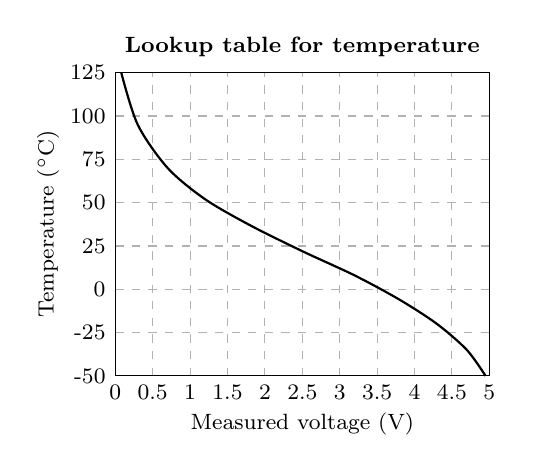
\begin{tikzpicture}[x=0.95cm,y=0.022cm,font=\footnotesize]
\node[font=\footnotesize\bfseries] at (2.5,140) {Lookup table for temperature};
\draw[gray!60,dashed] (0,-50) grid[xstep=0.5,ystep=25] (5,125);
\draw (0,-50) rectangle (5,125);
\foreach \x in {0,0.5,1,1.5,2,2.5,3,3.5,4,4.5,5} \node[below] at (\x,-50) {\x};
\foreach \y in {-50,-25,0,25,50,75,100,125} \node[left] at (0,\y) {\y};
\node[rotate=90] at (-0.9,37.5) {Temperature ($^\circ$C)};
\node at (2.5,-78) {Measured voltage (V)};
\draw[thick] plot[smooth] coordinates {(0.08,125) (0.3,95) (0.7,70) (1.2,52) (1.8,37) (2.5,22) (3.2,8) (3.8,-6) (4.3,-20) (4.7,-35) (4.95,-50)};
\end{tikzpicture}}}{01}{3}{\illegc}
\q{6.}{What happens if the battery is allowed for overcharging?}{01}{3}{\illegc}
\end{longtable}
\btfoot{|l|l|l|*{10}{C{0.85cm}|}}{\hline
\multirow{2}{*}{\shortstack{Marks\\Distribution}} & \multicolumn{2}{c|}{Particulars} & CO1 & CO2 & CO3 & CO4 & L1 & L2 & L3 & L4 & L5 & L6\\\cline{2-13}
 & Test & \shortstack{Max\\Marks} & - & 06 & 04 & - & 06 & 03 & 01 & - & \illegc & \illegc\\\hline}
\stars{***********}
\end{xpaper}

% ---------- 21CV75IF Integrated Health Monitoring of Structures
% (scan page 15 is a blurred shot of this paper; page 17 of the scan is the readable copy used here)
\begin{xpaper}
\par\vspace{2pt}\centerline{\sansfont\fontsize{12}{14}\selectfont Department of Civil Engineering}\par\vspace{8pt}
\ofour{29-01-2025}{50+10}{\textbf{21CV75IF}}{120 Min}{VII}{CIE -- II}{INTEGRATED HEALTH MONITORING OF STRUCTURES}
{\small Note: Answer all questions.}\par\vspace{3pt}
\begin{gtable}[QUIZ]{Sl.\newline No.}{Questions}{M}{BT}{CO}
\q{1}{Define smart materials in the context of Structural Health Monitoring (SHM)}{2}{1}{2}
\q{2}{What is Static field testing}{2}{1}{3}
\q{3}{List two Electric Field Sensors}{2}{1}{2}
\q{4}{List the Benefits of AI in SHM}{2}{1}{2}
\q{5}{Load cell can be used as \blank[1.8cm], \blank[1.8cm]}{2}{1}{2}
\end{gtable}
\begin{gtable}[TEST]{Sl.\newline No.}{Questions}{M}{BT}{CO}
\q{1}{With a neat sketch explain the evolution of materials used for structural health monitoring and its application .}{10}{3}{2}
\q{2}{Classify Smart Materials used in SHM with examples}{10}{3}{2}
\q{3}{Explain the different types of static load tests and conditions for its application}{10}{2}{3}
\q{4}{Discuss the sensor systems and hardware requirements in Static Field Testing}{10}{2}{3}
\q{5}{Explain the working Principle and advantage of EMI Technique for structural health monitoring}{10}{2}{2}
\end{gtable}
{\small\bfseries Course outcomes:}\par
\btfoot{|l|l|l|*{10}{C{0.8cm}|}}{\hline
\multirow{2}{*}{\shortstack{Marks\\Distribution}} & \multicolumn{2}{c|}{Particulars} & CO1 & CO2 & CO3 & CO4 & L1 & L2 & L3 & L4 & L5 & L6\\\cline{2-13}
 & Test & Max Marks & - & 38 & 22 & - & 10 & 30 & 20 & & & \\\hline}
\stars{***********}
\end{xpaper}

% ---------- 21CM75ID Advances in Corrosion Science and Management
\begin{xpaper}
\par\vspace{2pt}\centerline{\fontsize{14}{16}\selectfont Academic year 2024-2025 (Odd Sem)}\par\vspace{2pt}
\centerline{\bfseries\fontsize{14}{16}\selectfont (CIE-II FOR VII SEM)}\par\vspace{8pt}
\centerline{\bfseries DEPARTMENT OF CHEMISTRY}\par\vspace{2pt}
\noindent\begingroup\renewcommand{\arraystretch}{1.25}\fontsize{11.5}{13}\selectfont
\begin{tabular}{|C{3.6cm}|C{4.4cm}|C{4.2cm}|C{3.8cm}|}\hline
Date & 29.01.2025 & Sem - VII & CIE-II\\\hline
Course Code & 21CM75ID & Maximum Test Marks & \shortstack{Quiz-10 + Test-50\\(60M)}\\\hline
Course Name & ACSM & Duration & 120 mins\\\hline
\multicolumn{4}{|c|}{\bfseries ADVANCES IN CORROSION SCIENCE AND MANAGEMENT}\\\hline
\end{tabular}\endgroup\par\vspace{6pt}
{\bfseries Note: 1) Answer all the questions}\par
\hspace*{1.05cm}{\bfseries 2) \ Part A should be answered in the first two pages of the answer script.}\par\vspace{6pt}
\begin{longtable}{|C{1.05cm}|p{12.2cm}|C{0.95cm}|C{0.95cm}|C{0.95cm}|}
\hline & \multicolumn{1}{c|}{\textbf{Part-A}} & \textbf{M} & \textbf{BTL} & \textbf{CO}\\\hline
\q{1}{What is the impact of substrate temperature on the PVD (sputtering) process?}{1}{4}{2}
\q{2}{How does the alkalinity of an environment influence the interpretation of Pourbaix diagrams?}{1}{3}{2}
\q{3}{What is the role of resin in varnish?}{1}{2}{1}
\q{4}{How do you differentiate between varnish and enamel?}{1}{3}{3}
\q{5}{Chromium anodes are not used in the process of chrome plating. Justify}{1}{3}{2}
\q{6}{What are oxygen scavengers?}{1}{2}{1}
\q{7}{Identify the missing product in the following reaction concerning the electroless plating of Nickel.\par\vspace{2pt}
\hspace*{0.5cm}H$_2$PO$_2^-$ + H$_2$O + Ni$^{+2}$ \ $\Longrightarrow$ \ \ ? \ + 2H$^+$ + Ni}{1}{4}{2}
\q{8}{Write the electrolytic bath composition of Nickel plating.}{1}{1}{2}
\q{9}{Name the film-forming material in paint.}{1}{1}{2}
\q{10}{List any one limitation of the Pourbaix diagram.}{1}{1}{3}
\end{longtable}
\par\vspace{8pt}
\begin{longtable}{|C{1.05cm}|p{12.2cm}|C{0.95cm}|C{0.95cm}|C{0.95cm}|}
\hline & \multicolumn{1}{c|}{\textbf{Part-B}} & \textbf{M} & \textbf{BTL} & \textbf{CO}\\\hline
\q{11}{Outline the methods by which corrosion inhibitors function to reduce corrosion rates in metal structures. Explain with reactions.}{7}{2}{2}
\q{12}{For the oxygen reduction reaction\newline
O$_2$(g) + 4 H$^+$ (aq) + 4e$^-$ $\longleftrightarrow$ 2H$_2$O (l)\newline
The standard electrode potential (Eo) is +1.23 V. Calculate the equilibrium potential at pH= 7, where the concentration of oxygen is 0.21 atm. Interpret the result obtained.}{7}{3}{3}
\q{13}{What are the key differences between electroless plating and electroplating? Explain the process of copper electroplating with reactions.}{7}{\illegc}{\illegc}
\q{14}{List out the main components of paints. Explain any 3 components with examples along with their role.}{7}{\illegc}{\illegc}
\q{15}{How can corrosion be controlled through effective design? Analyze and interpret the role of design in corrosion control concerning practical situations. what is the clarity of this question}{7}{\illegc}{\illegc}
\q{16}{An experiment involved two aluminum samples, each with an initial weight of 200 grams. One sample was treated with a corrosion inhibitor, while the other remained untreated. After exposure to a marine environment for 30 days, the treated sample's final weight was 198 grams, and the untreated sample's final weight was 195 grams. Given the density of aluminum is 2.7 g/cm\textsuperscript{3} and the constant K is 87.6, calculate the corrosion rate for each sample using the weight loss method, expressed in millimeters per year (mmpy). Compare and interpret the results to determine the effectiveness of the corrosion inhibitor.}{7}{3}{\illegc}
\q{17}{Construct a Pourbaix diagram for Aluminium, assuming the activity of all dissolved substances is 10$^{-6}$ M at room temperature (298K). Using the diagram, interpret the corrosion tendency of Aluminium under different conditions, including the relevant electrochemical reactions. Discuss practical solutions for mitigating Aluminium corrosion based on your diagram analysis.}{8}{3}{\illegc}
\end{longtable}
\xfoot{BT-Blooms Taxonomy, CO-Course Outcomes, M-Marks}{|l|l|*{8}{C{0.85cm}|}l|}{\hline
\multirow{2}{*}{\shortstack{Marks\\Distribution}} & Particulars & CO1 & CO2 & CO3 & CO4 & L1 & L2 & L3 & L4 & \multirow{2}{*}{\illeg\ (cut off in the scan)}\\\cline{2-10}
 & Max Marks & 16 & 13 & 16 & 15 & 4 & 16 & 25 & 15 & \\\hline}
\stars{************************}
\end{xpaper}

% ---------- 21ME75IQ Nuclear Engineering
\begin{xpaper}
\par\vspace{2pt}\centerline{\itshape\fontsize{12}{14}\selectfont Department of Mechanical Engineering}\par\vspace{4pt}
\noindent\begingroup\renewcommand{\arraystretch}{1.5}\fontsize{11.5}{13}\selectfont
\begin{tabular}{|C{3.5cm}|C{4.6cm}|C{3.9cm}|C{4.1cm}|}\hline
Date & \textbf{29 January 2025} & Maximum Marks & Quiz 10 + Test 50\\\hline
Course Code & \textbf{21ME75IQ} & Duration & 120 Min\\\hline
Course Name & \textbf{Nuclear Engineering} & \multicolumn{2}{l|}{\textbf{USN:}}\\\hline
\end{tabular}\endgroup\par\vspace{8pt}
\begin{longtable}{|C{1.05cm}|p{14.3cm}|C{0.8cm}|}
\hline \textbf{Q} & \multicolumn{1}{c|}{\textbf{PART-A (Quiz)}} & {\scriptsize M}\\\hline
\qm{1.1}{Calculate the binding energy of an alpha particle if mass of $^1_1$H atom is 1.007826 u, mass of neutron is 1.008665 u, mass of $^4_2$He atom is 4.00260 u. Take 1 u = 931 MeVc$^{-2}$ .}{1}
\qm{1.2}{Find the increase in mass of water when 1 kg of water absorbs 4.2 $\times$ 10$^3$ J of energy to produce a temperature rise of 1 K.}{1}
\qm{1.3}{The binding energy of $^{35}_{17}$Cl nucleus is 298 MeV. Calculate its approximate atomic mass. Given that, mass of proton is m$_\mathrm{p}$ = 1.007825 amu and mass of neutron is m$_\mathrm{n}$ = 1.008665 amu.}{1}
\qm{1.4}{The electric potential energy (in \textbf{MeV}) of interaction due to the electric repulsion between two nuclei of $^{12}$C when they touch each other at the surface is given by\ldots\ldots\ Assume that the potential energy of interaction between two nuclei is given by U = $\frac{1}{4\pi\epsilon_0}\frac{Q_1Q_2}{r}$ .}{1}
\qm{1.5}{A radioactive nucleus X decays to a stable nucleus Y. Then the graph of rate of formation of Y against time t will be given as}{1}
\qm{1.6}{A nucleus X initially at rest, undergoes alpha decay according to the equation $^{232}_{\ Z}$X $\rightarrow$ $^{A}_{90}$Y + $\alpha$. What fraction of the total energy released in the decay will be the kinetic energy of the alpha particle?}{1}
\qm{1.7}{At time t = 0, N$_1$ nuclei of decay constant $\lambda_1$ and N$_2$ nuclei of decay constant $\lambda_2$ is mixed. The decay rate of mixture is}{1}
\qm{1.8}{Sun radiates energy in all direction. The average energy received at earth is 1.4 kWm$^{-2}$. The average distance between the earth and the sun is 1.5 $\times$ 10$^{11}$ m. If this energy is released by conservation of mass into energy, then the mass lost per day by the sun is approximately}{1}
\qm{1.9}{Nuclei of radioactive element A are produced at a rate t$^2$ at any time t. The element A has decay constant $\lambda$ . Let N be the number of nuclei of element A at any time t. At time t = t$_0$, dN/dt is minimum. Then the number of nuclei of element A at time t = t$_0$ is}{1}
\qm{1.10}{In a radioactive decay, let \textit{N} represent the number of residual active nuclei, \textit{D} the number of daughter nuclei, and \textit{R} the rate of decay at any time \textit{t}. Three curves are shown in figure. The correct ones are\par\vspace{4pt}
\begin{tikzpicture}[x=1cm,y=1cm,font=\scriptsize,>=Latex]
\draw[->] (0,0)--(1.9,0) node[right]{$t$}; \draw[->] (0,0)--(0,1.5) node[above]{$N$}; \node at (0.9,0.75) {\tiny\textit{[curve illegible]}}; \node at (0.9,-0.35) {(1)};
\begin{scope}[xshift=3cm]\draw[->] (0,0)--(1.9,0) node[right]{$t$}; \draw[->] (0,0)--(0,1.5) node[above]{$D$}; \draw (0,0) .. controls (0.3,0.9) and (0.7,1.05) .. (1.4,1.1); \node at (0.9,-0.35) {(2)};\end{scope}
\begin{scope}[xshift=6cm]\draw[->] (0,0)--(1.9,0) node[right]{$t$}; \draw[->] (0,0)--(0,1.5) node[above]{$\frac{R}{N}$}; \draw (0,1.0)--(1.4,1.0); \node at (0.9,-0.35) {(3)};\end{scope}
\end{tikzpicture}}{1}
\end{longtable}
\par\vspace{10pt}
\centerline{\itshape\fontsize{12}{14}\selectfont Department of Mechanical Engineering}\par\vspace{6pt}
\begin{longtable}{|C{1.05cm}|p{14.3cm}|C{0.8cm}|}
\hline \textbf{Q} & \multicolumn{1}{c|}{\textbf{PART-B (Test)}} & {\scriptsize M}\\\hline
\qm{1}{In an nuclear lab an experiment is conducted and following result is observed: A radionuclide with half life 1620 sec is produced at a constant rate 1000 nuclei per second. During each decay energy 200 MeV is released. If production of radio nuclides started at t = 0, calculate
\begin{rom}\item the rate of release of energy at 3240 second and\item the total energy released upto 405 second.\end{rom}}{10}
\qm{2}{During an EL presentation on nuclear engineering topic at RVCE to determine the half-life of a radioactive nuclide a group of students shown the graph of ln$\left|\frac{dN(t)}{dt}\right|$ versus t as shown below. It was mentioned that ln$\left|\frac{dN(t)}{dt}\right|$ represents the rate of radioactive decay at time t. If the number of radioactive nuclei of this element decreases by a factor of \textit{p} after 4.16 yr , then what was the calculated value of \textit{p}?\par\vspace{4pt}
\centerline{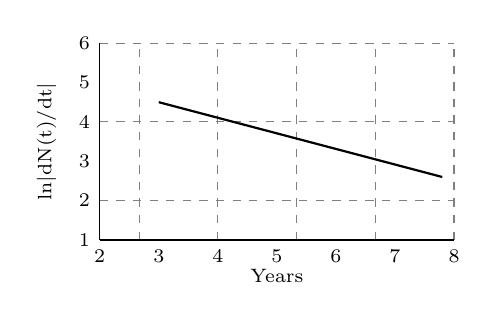
\begin{tikzpicture}[x=0.75cm,y=0.5cm,font=\scriptsize]
\draw[dashed,gray] (2,1) grid (8,6); \draw (2,1)--(8,1); \draw (2,1)--(2,6);
\foreach \x in {2,...,8} \node[below] at (\x,1) {\x}; \foreach \y in {1,...,6} \node[left] at (2,\y) {\y};
\node at (5,0.1) {Years}; \node[rotate=90] at (1.1,3.5) {ln$|$dN(t)/dt$|$};
\draw[thick] (3,4.5)--(7.8,2.6);
\end{tikzpicture}}}{10}
\qm{3}{For a radioactive material, its activity \textit{A} and rate of change of its activity R are defined as A = $-\frac{dN}{dt}$ and R= $-\frac{dA}{dt}$, where \textit{N}(\textit{t}) is the number of nuclei at time \textit{t} . Two radioactive source \textit{P} (mean life, $\tau$) and \textit{Q} (mean life, 2$\tau$) have the same activity at \textit{t} = 0 . Their rate of change of activities at \textit{t} = 2$\tau$ are R$_P$ and R$_Q$ , respectively. If $\frac{R_P}{R_Q}=\frac{z}{e}$, calculate the value of z.}{10}
\qm{4}{The $\beta$-particles and $\gamma$-decays happens as shown in the figure below:\par\vspace{4pt}
\centerline{\begin{tikzpicture}[x=1cm,y=1cm,font=\footnotesize,>=Latex]
\draw (0,3)--(4.5,3) node[pos=0,left]{$_{12}$Mg$^{27}$};
\draw (2.1,0.9)--(4.5,0.9) node[right]{1.015 MeV};
\draw (1.4,0.6)--(4.5,0.6) node[right]{0.834 MeV};
\draw (0,0)--(4.5,0) node[pos=0,left]{$_{13}$Al$^{27}$} node[right]{0};
\draw[->] (0.3,3)--(1.9,0.6) node[pos=0.45,right]{$\beta_2^-$};
\draw[->] (2.9,3)--(4.0,0.9) node[pos=0.45,left]{$\beta_1^-$};
\draw[->] (4.2,0.9)--(4.2,0.6) node[midway,right]{$\gamma_1$};
\draw[->,decorate,decoration={snake,amplitude=1pt,segment length=4pt}] (2.6,0.9)--(2.6,0) ; \node at (2.95,0.75) {$\gamma_2$};
\draw[->] (2.0,0.6)--(2.0,0) node[midway,left]{$\gamma_3$};
\end{tikzpicture}}\par\vspace{2pt}
Find the kinetic energy of $\beta$-particles and radiation frequencies of $\gamma$-decay.\newline
Given that mass of $^{27}_{12}$\textit{Mg} atom is 26.991425 u and mass of $^{27}_{13}$\textit{Al} atom is 26.990080 u.}{10}
\qm{5}{The nucleus X is unstable was initially at rest and after decay of an $\alpha$-particle becomes stable Y nucleus as shown: $^{228}_{\ 92}$X $\rightarrow$ $^{A}_{90}$Y + $\alpha$. At \textit{t} = 0, the emitted particle enters in a region of space where a uniform magnetic field $\vec{B}$ = B$_o\hat{i}$ and electric field $\vec{E}$ = E$_o\hat{i}$ exist. The $\alpha$-particle enters in the region with velocity $\vec{V}$ = V$_o\hat{j}$ from x = 0. At time t = $(\sqrt{3}\times10^7)\left\{\frac{m_\alpha}{q_\alpha E_o}\right\}$ seconds, the particle was observed to have speed twice the initial speed v$_0$ , then find (a) the velocity of a particle at time \textit{t}. (b) the initial velocity v$_0$ of the $\alpha$-particle, (c) the binding energy per nucleon of $\alpha$-particle. Given that: \textit{m}(\textit{Y}) = 221.03 u, \textit{m}($\alpha$) = 4.003 u, \textit{m}(\textit{n}) = 1.009 u, \textit{m}(\textit{p}) = 1.008 u, \textit{m}$_\alpha$ = (2/3)$\times$ 10$^{-26}$ kg, \textit{q}$_\alpha$ = 3.2 $\times$ 10$^{-19}$ C and 1 u = 931 MeVc$^{-2}$}{10}
\end{longtable}
\stars{All the best!}
\stars{*******}
\end{xpaper}

% ---------- 21CH751C Sustainability and Life Cycle Analysis (Institutional Elective)
\begin{iempaperB}
\paperinfo{ayear={2024-2025 (Odd Sem)},usn=0,dept={CHEMICAL ENGINEERING},date={29\textsuperscript{th} Jan 2025},code={21CH751C},sem={VII Semester},exam={CIE 2},maxmarks={60},duration={120 Min},
 title={SUSTAINABILITY AND LIFE CYCLE ANALYSIS (Institutional Elective)},shownote=0}
\iemheadB
{\small\bfseries Note: 1. \ Answer all the Questions.}\par\vspace{3pt}
\begin{longtable}{|C{0.5cm}|C{0.5cm}|p{12.15cm}|C{0.95cm}|C{0.95cm}|C{0.95cm}|}
\hline \multicolumn{3}{|c|}{\textbf{Part A}} & \textbf{M} & \textbf{BT} & \textbf{CO}\\\hline
1 & a & Name the frame works used for the identification and structuring of environment indicators. & 1 & 1 & 2\\\hline
 & b & Name the technique that can detect most of the elements of periodic table. & 1 & 1 & 2\\\hline
 & c & Identify the component of a hair dryer that has the highest environmental impact. & 1 & 3 & 3\\\hline
 & d & Define traditional engineering. & 1 & 1 & 3\\\hline
 & e & List two contradictions of LCA. & 1 & 1 & 2\\\hline
 & f & State Sherwood relationship. & 1 & 1 & 2\\\hline
 & g & Name one each government data base and commercial data base available for LCA & 2 & 1 & 1\\\hline
 & h & Analyze and calculate the ratio of the abundance of materials in the Earth's crust (tons) to the annual use of the materials (tons/yr). Assume an approximate for the crust of 2 x 10\textsuperscript{19} metric tons. This mass is based on a 40 km thickness for continental crust and a 3 km thickness for oceanic crust, with an average density of 3 g/cm\textsuperscript{3} (3 tons/m\textsuperscript{3}). The availability of P in abundance is 0.1\% and its usage of Tons/Year is 1.53 x10\textsuperscript{6}. & 2 & 4 & 2\\\hline
\multicolumn{3}{|c|}{\textbf{Part B}} & & & \\\hline
 & & List the components of LCA and explain the LCA process in detail. & 10 & 2 & 3\\\hline
2 & a & With a neat diagram explain Inductively coupled plasma atomic emission spectroscopy ICP AES & 07 & 2 & 4\\\hline
 & b & List the steps of toxicity characteristic leaching procedure. & 03 & 1 & 2\\\hline
3 & a & With a neat diagram explain the sustainable development and design thinking. & 07 & 2 & 3\\\hline
 & b & Explain the three-pronged approach to characterize the foot print & 03 & 2 & 2\\\hline
4 & & Construct an explanation of the chemistry of dry gasification. & 10 & 3 & 3\\\hline
5 & & Analyze the parameters of sustainability and explain why stone, leather, metals, and timber are regarded as sustainable materials. & 10 & 4 & 4\\\hline
\end{longtable}
\stars{\makebox[\textwidth]{\dotfill}}
\end{iempaperB}

% ---------- 21CS75IE Prompt Engineering (Institutional Electives - II, Group G)
\begin{iempaperB}
\paperinfo{ayear={2024-2025 (Odd Sem)},usn=0,dept={COMPUTER SCIENCE AND ENGINEERING},date={Jan 2025},code={21CS75IE},sem={07},exam={CIE-II},maxmarks={10+50},duration={120 Min},
 title={PROMPT ENGINEERING \ {\normalfont( INSTITUTIONAL ELECTIVES -- II (Group G))}},shownote=0}
\iemheadB
\begin{longtable}{|C{1.05cm}|p{12.2cm}|C{0.95cm}|C{0.95cm}|C{0.95cm}|}
\hline \textbf{Q. No.} & \centering\textbf{Questions}\newline\textbf{QUIZ} & \textbf{M} & \textbf{BT} & \textbf{CO}\\\hline
\qq{}{1.1 \ Give one example where few-shot learning can be used in LLM applications}{01}{1}{1}
\qq{}{1.2 \ Name one external tool commonly used with LLMs for real-time data retrieval.}{01}{2}{2}
\qq{}{1.3 \ Which API would be useful for integrating weather data into an LLM application}{01}{2}{2}
\qq{}{1.4 \ What is the benefit of using an external database for LLM-based question-answering tasks ?}{01}{1}{1}
\qq{}{1.5 \ What type of external data would improve the performance of an LLM used for financial predictions ?}{01}{1}{1}
\qq{}{1.6 \ Which factor is crucial for the successful deployment of prompts in production environments ?}{01}{1}{1}
\qq{}{1.7 \ Give one example of a task where information extraction from social media could be useful?}{01}{1}{2}
\qq{}{1.8 \ What does ``NER'' stand for in the context of information extraction?}{01}{2}{1}
\qq{}{1.9 \ Provide an example of an entity that could be extracted from the sentence ``Schedule a meeting with John tomorrow at 3 PM}{01}{1}{1}
\q{}{1.10 \ In the context of API integration, what does REST stand for ?}{01}{1}{1}
\q{}{\centering TEST}{}{}{}
\q{2.}{Summarization using sources is an essential task for LLMs. How can LLMs leverage external sources to generate more precise and reliable summaries? Discuss the methodology for retrieving relevant information from external data sources, synthesizing it, and generating a coherent summary. Provide examples from industri\illeg}{10}{1}{1}
\q{3.}{Explain the best practices in prompt engineering for large language models (LLMs). Discuss how prompt design influences model performance and how to craft clear, specific, and concise prompts for effective results. Provide examples of both effective and ineffective prompts.}{10}{1}{2}
\q{4.}{Advanced prompting techniques often involve the combination of multiple approaches. Discuss how advanced prompting methods like few-shot learning, zero-shot learning, and chain-of-thought prompting are applied in real-world scenarios. Compare their effectiveness and challenges in different use cases.\newline task without any explicit examples, relying solely on the clarity of the instructions.}{10}{4}{5}
\q{5.}{Explain the role of information extraction in function calling. How can a conversational agent extract specific information (such as dates, times, and names) from user input, and how does it invoke functions to act on this extracted data?}{10}{3}{4}
\q{6.}{Explain the different techniques used in document parsing for information extraction. How can complex documents such as contracts, financial statements, and academic papers be parsed to extract meaningful information for automation and decision-making processes?}{10}{2}{3}
\end{longtable}
\stars{***********}
\xfoot{BT-Blooms Taxonomy, CO-Course Outcomes}{|l|l|l|*{10}{C{0.85cm}|}}{\hline
\multirow{2}{*}{\shortstack{Marks\\Distribution}} & \multicolumn{2}{c|}{Particulars} & CO1 & CO2 & CO3 & CO4 & L1 & L2 & L3 & L4 & L5 & L6\\\cline{2-13}
 & \shortstack{Test \&\\Quiz} & \shortstack{Max\\Marks} & 17 & 13 & 10 & 10 & 10 & 27 & 13 & 10 & - & -\\\hline}
\cotable{Course Outcomes:}{CO1: & Demonstrate an understanding of prompt engineering principles including how prompt structure and phrasing impact the performance of AI models.\\\hline
CO2: & Design and implement effective prompts- to create and apply prompts for various natural language processing (NLP) tasks, such as text generation, summarization, and translation, using AI models..\\\hline
CO3: & Critically evaluate the effectiveness of prompts - assess the quality and performance of prompts in terms of accuracy, coherence, and relevance, identifying \illeg\\\hline
CO4: & Apply prompt engineering \illeg\ (rest of the page is cut off in the scan)}
\end{iempaperB}

% ---------- 21HS75IR Principles & Practices of Cyber Law
\begin{iempaperB}
\paperinfo{ayear={2024-2025 (ODD Sem)},usn=0,date={29/01/2025},code={21HS75IR},sem={VII},exam={CIE -- II},maxmarks={10+50},duration={120 Mins},
 title={PRINCIPLES \& PRACTICES OF CYBER LAW},shownote=0}
\iemheadB
\onenote{Answer all the Questions.}
\begin{longtable}{|C{1.05cm}|p{12.2cm}|C{0.95cm}|C{0.95cm}|C{0.95cm}|}
\hline Q.No. & \multicolumn{1}{c|}{\textbf{PART- A}} & M & BT & CO\\\hline
\q{1}{List any two types of E-commerce models.}{2}{2}{CO2}
\q{2}{What are `Digital Signature' and its use in E-commerce?}{2}{2}{CO2}
\q{3}{What is the main concern regarding copyright infringement in cyberspace?}{2}{2}{CO3}
\q{4}{How does cybersquatting affect trademark owners?}{2}{2}{CO3}
\q{5}{How can a trademark owner protect their brand online?}{2}{2}{CO4}
\qpart{PART -B}
\q{1}{A company named XYZ Ltd. enters into a contract with ABC Ltd. through an online platform. The contract is electronically signed by representatives of both parties using Digital Signatures issued by a recognized Certifying Authority. However, later, XYZ Ltd. disputes the validity of the contract, claiming that one of the signatories had not authorized the use of their digital signature.\newline
(i)What role does a Digital Signature play in validating an electronic contract?\newline
(ii)What legal provisions under the IT Act 2000 support the enforceability of this electronic contract?}{10}{4}{CO2}
\q{2}{A company launches a new product and discovers a similar domain name being used to divert customers to a competitor's site. Propose a comprehensive strategy to address this issue legally and technologically with one case example.}{10}{4}{CO2}
\q{3}{Bring out the difference between Digital Signature \& Electronic Signature along with the advantages and disadvantages.}{10}{2}{CO3}
\q{4}{Design a comprehensive strategy for an e-commerce business to protect customer transactions using digital signatures and cryptography.}{10}{3}{CO4}
\q{5a}{If an individual finds that their copyrighted work has been uploaded to a website without their consent, what steps should they take to protect their rights.}{05}{2}{CO4}
\q{5b}{Analyze the impact of piracy on digital content creators in cyberspace.}{05}{2}{CO2}
\end{longtable}
\btfoot{|l|l|l|*{10}{C{0.8cm}|}}{\hline
\multirow{2}{*}{Marks Distribution} & \multicolumn{2}{c|}{Particulars} & CO1 & CO2 & CO3 & CO4 & L1 & L2 & L3 & L4 & L5 & L6\\\cline{2-13}
 & Test & Max Marks & 30 & 30 & & & & 20 & 10 & 20 & & \\\hline}
\end{iempaperB}

% ---------- 21IM78 Innovation and Entrepreneurship
\begin{iempaperB}
\paperinfo{ayear={2024-2025 (ODD Sem)},date={28.01.2025},code={21IM78},sem={VII Semester},exam={CIE -- II},maxmarks={05 + 25},duration={60 Mins},
 title={INNOVATION AND ENTREPRENEURSHIP},shownote=0}
\iemheadB
{\small Note:}\par\vspace{-1pt}
\hspace*{0.5cm}{\footnotesize 1. \hspace{0.1cm}Answer all the Questions.}\par
\hspace*{0.5cm}{\footnotesize 2. \hspace{0.1cm}Use suitable sketches and tabular column wherever necessary.}\par
\hspace*{0.5cm}{\footnotesize 3. \hspace{0.1cm}Observe the marks split-up and answer accordingly.}\par\vspace{3pt}
\begin{gtable}[PART -- A]{Sl.\newline No.}{Questions}{M}{BT}{CO}
\q{1}{List any two rules of brainstorming.}{01}{L1}{CO1}
\q{2}{Imagine you are starting your ice-cream outlet. List 2 ways in which you can make sure your funds are used optimally.}{01}{L2}{CO2}
\q{3}{Identify two bad practices students are doing to get ``AICTE activity points''. Suggest two methods to curtail the same.}{02}{L4}{CO2}
\q{4}{Comment on the importance of ``Early Adopters''.}{01}{L3}{CO3}
\end{gtable}
\begin{gtable}[PART -- B]{Sl.\newline No.}{Questions}{M}{BT}{CO}
\q{1.}{Discuss the four types of Markets (Use tabular column format) and comment on the most suitable market type for a start-up venture.}{05}{L2}{CO2}
\q{2.}{When you are allowed to form teams on your own, lack of coordination among the team members is clearly visible and reflects in the outcome of the work also. As individuals, each of the students is competent in their own way. Use design thinking principles to identify the problem with students and how it can be resolved. (Concentration should be on the first three stages of DT)}{05}{L4}{CO3}
\q{3.}{Illustrate the lean canvas of business model for your practice venture using Ash Maurya's template and assess each of the 9 blocks using a 5-point scale (1 being lowest and 5 being highest). Identify any 3 blocks which needs improvements and suggest strategies to improve the same.}{05}{L3}{CO4}
\q{4.}{Construct 2 detailed personas of students belonging engineering education from your college and propose 2 problem definitions using DT framework.}{07}{L5}{CO3}
\q{5.}{Choose any 1 problem definition from the previous question and answer the following.
\begin{romi}\item Assess \& depict the input requirements based on your understanding the solution space. (2 marks)\item Sketch the solution. (1 mark)\end{romi}}{03}{L5}{CO4}
\end{gtable}
\btfoot{|l|l|l|*{5}{C{0.8cm}|}*{6}{C{0.8cm}|}}{\hline
\multirow{3}{*}{Marks} & \multicolumn{2}{c|}{Particulars} & CO1 & CO2 & CO3 & CO4 & CO5 & L1 & L2 & L3 & L4 & L5 & L6\\\cline{2-14}
 & \multirow{2}{*}{\shortstack{Max\\Marks}} & Quiz & 01 & 03 & 01 & -- & -- & 01 & 01 & 01 & 02 & -- & --\\\cline{3-14}
 & & Test & -- & 05 & 12 & 08 & -- & -- & 05 & 05 & 05 & 10 & --\\\hline}
\stars{*****}
\end{iempaperB}

\end{document}
